
%(BEGIN_QUESTION)
% Copyright 2008, Tony R. Kuphaldt, released under the Creative Commons Attribution License (v 1.0)
% This means you may do almost anything with this work of mine, so long as you give me proper credit

A piece of laboratory equipment uses a voltage divider to reduce voltage to two electromagnet coils from a higher-voltage source.  Coil \#1 is supposed to receive 2.91 volts and coil \#2 is supposed to receive 13.11 volts:

$$\includegraphics[width=15.5cm]{i03166x01.eps}$$

One day, something goes wrong with this circuit.  The magnetic field from coil \#1 suddenly disappears, yet there is still a magnetic field coming from coil \#2.  The technician who looked at this problem before you took two voltage measurements and then gave up: 13.55 volts at test point TP3 and 5.42 volts at test point TP4.  You left your multimeter back at the shop, which means you cannot take any more voltage measurements.  However, since you are more determined than the former technician, you proceed to identify the following from the two measurements already taken:

\vskip 10pt

\begin{itemize}
\item{} \underbar{Two} components or wires in the circuit that you know cannot be failed either open or shorted, besides the 24 volt source which is obviously operational.
\vskip 40pt
\item{} \underbar{One} component or wire in the circuit you think could possibly be bad, and the type of failure it would be (either open or shorted).
\end{itemize}

\vfil 

\underbar{file i03166}
\eject
%(END_QUESTION)





%(BEGIN_ANSWER)

This is a graded question -- no answers or hints given!

%(END_ANSWER)





%(BEGIN_NOTES)

Since we know coil \#2 is still generating a magnetic field, there must still be current going through it.  This means we must have continuity all the way from the source through to coil \#2.

\vskip 10pt

The fact that coil \#1 is not outputting a magnetic field, and that the voltage between TP4 and ground is much greater than it should be, tells us that there must be an ``open'' fault interrupting current through coil \#2 (a ``shorted'' fault there would {\it decrease} voltage at TP4 rather than increase it).  Thus, we may draw the following conclusions regarding good and potentially faulted components:

\vskip 10pt

\goodbreak
\noindent
{\bf Components known to be in good working condition:}

\begin{itemize}
\item{} Wire from battery to $R_1$
\item{} Wire from TP2 to TP3
\item{} $R_1$
\item{} $R_2$
\item{} $R_3$
\item{} Coil \#2
\end{itemize}

\vskip 10pt

\goodbreak
\noindent
{\bf Components which could possibly be faulted:}

\begin{itemize}
\item{} Wire from TP4 to TP5 broken (open)
\item{} Coil \#1 failed open
\end{itemize}

%INDEX% Troubleshooting review: electric circuits

%(END_NOTES)


